 \iffalse
\let\negmedspace\undefined
\let\negthickspace\undefined
\documentclass[journal,12pt,twocolumn]{IEEEtran}
\usepackage{cite}
\usepackage{amsmath,amssymb,amsfonts,amsthm}
\usepackage{algorithmic}
\usepackage{graphicx}
\usepackage{textcomp}
\usepackage{xcolor}
\usepackage{txfonts}
\usepackage{listings}
\usepackage{enumitem}
\usepackage{mathtools}
\usepackage{gensymb}
\usepackage{comment}
\usepackage[breaklinks=true]{hyperref}
\usepackage{tkz-euclide} 
\usepackage{listings}
\usepackage{gvv} 
\usepackage{caption}
\def\inputGnumericTable{}                   

%\usepackage[latin1]{inputenc}                                
\usepackage{color}                                            
\usepackage{array}                                            
\usepackage{longtable}                                       
\usepackage{calc}                                             
\usepackage{multirow}                                         
\usepackage{hhline}                                           
\usepackage{ifthen}                                           
\usepackage{lscape}
\usepackage{tikz}
\newtheorem{theorem}{Theorem}[section]
\newtheorem{problem}{Problem}
\newtheorem{proposition}{Proposition}[section]
\newtheorem{lemma}{Lemma}[section]
\newtheorem{corollary}[theorem]{Corollary}
\newtheorem{example}{Example}[section]
\newtheorem{definition}[problem]{Definition}
\newcommand{\BEQA}{\begin{eqnarray}}
\newcommand{\EEQA}{\end{eqnarray}}
\newcommand{\define}{\stackrel{\triangle}{=}}
\theoremstyle{remark}
\newtheorem{rem}{Remark}

\begin{document}

\bibliographystyle{IEEEtran}
\vspace{3cm}

\title{GATE: EE - 11.2022}
\author{EE23BTECH11013 - Avyaaz$^{*}$% <-this % stops a space 
}
\maketitle
\newpage
\bigskip

\renewcommand{\thefigure}{\arabic{figure}}
\renewcommand{\thetable}{\arabic{table}}

\large\textbf{\textsl{Question:}}
The transfer function of a real system $H(S)$ is given as:
\begin{align}
    H(s) = \frac{As + B}{s^2 + Cs + D}\nonumber
\end{align}
where $A, B, C$ and $D$ are positive constants. This system cannot operate as
\begin{enumerate}[label={(\Alph*)}]
    \item Low pass filter
    \item High pass filter
    \item Band pass filter
    \item An Integrator
\end{enumerate}\hfill(GATE EE 11 2022) \\
\solution
\fi
The transfer function $H(s)$ is given by: 
\begin{align}
    H(s) = \frac{As + B}{s^2 + Cs + D}\label{eq:given.EE.11.2022}
\end{align}
Put $s = j\omega$ in \eqref{eq:given.EE.11.2022}:
\begin{align}
    H(j\omega) = \frac{A(j\omega) + B}{(j\omega)^2 + C(j\omega) + D} \\
    |H(j\omega)| = \frac{\sqrt{(A\omega)^2 + B^2}}{\sqrt{(D - \omega^2)^2 + (\omega C)^2}}\label{eq:magnitude.EE.11.2022}
\end{align}


\begin{table}[htbp]
\setlength{\extrarowheight}{4pt}
\setlength{\tabcolsep}{3pt}
\centering
\begin{tabular}{|c|c|}
\hline
\textbf{Parameter} & \textbf{Description}\\
\hline 
Low Pass Filter & The gain should be finite at low frequency  \\
\hline
High Pass Filter &The gain should be finite at high frequency \\
\hline
Band Pass Filter& Finite gain over frequency band \\
\hline
Integrator & Transfer function should have at least\\& one pole at origin \\
\hline
\end{tabular}

\caption{Conditions}
\label{tab:inputs.EE.11.2022}
\end{table}
% \item \noindent From \tabref{tab:inputs.EE.11.2022} and equation \eqref{eq:magnitude.EE.11.2022}:
\begin{enumerate}[label={\alph*)}]
    \item Low Pass Filter:
    
  At low frequency $(\omega = 0 )$:
 \begin{align}
     |H(\omega = 0)| = \frac{B}{D}\label{eq:lowpass.EE.11.2022}
 \end{align}
$\therefore$ H(s) can operate as Low pass filter.

\item High Pass Filter:

% From \tabref{tab:inputs.EE.11.2022} and equation \eqref{eq:magnitude.EE.11.2022}:

At high frequency $(\omega = \infty )$:
 \begin{align}
     |H(\omega = \infty)| = 0 \label{eq:highpass.EE.11.2022}
 \end{align}
 % From \tabref{tab:inputs.EE.11.2022}:
 
$\therefore$ $H(s)$ cannot operate as High pass filter.
\item Band Pass Filter:

 Assuming B is a very less positive valued constant as compared to others:
\begin{align}
        |H(j\omega)| = \frac{(A\omega)}{\sqrt{(D - \omega^2)^2 + (\omega C)^2}}\\
   \implies      |H(\omega = 0)| = 0 \text{ and }  |H(\omega = \infty)| = 0 \label{eq:bandpass.EE.11.2022}
\end{align}

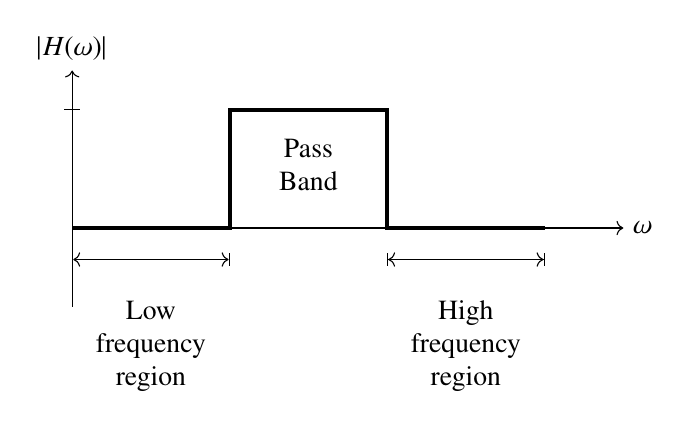
\begin{tikzpicture}
  
    \draw[->] (0,0) -- (7,0) node[right] {$\omega$};
   
    \draw[->] (0,-1) -- (0,2) node[above] {$|H(\omega)|$};
  
    \draw[line width=1.5pt]  (0,0) -- (2,0) -- (2,1.5) -- (4,1.5) -- (4,0) --(6,0);
    \draw[-]{(0,1.5)};
      \draw (-0.1,1.5) -- (0.1,1.5);
         \draw[|<->|]{(0,-0.4) -- (2,-0.4)};
    \node[align=center] at (1,-1.5) {Low \\frequency\\ region};
         \draw[| <-> |]{(4,-0.4) -- (6,-0.4)};
    \node[align=center] at (5,-1.5) {High \\frequency\\ region};
    \node[align=center] at (3,0.8) {Pass\\Band};

\end{tikzpicture}
$\because$ $H(s)$ passes frequency between low and high frequencies.

$\therefore$ $H(s)$ can operate as a band pass filter.
\item Integrator:

At very high value of frequency$(\omega\mkern-4mu \rightarrow\mkern-6mu\infty)$:
\begin{align}
    H(s) \approx \frac{As}{s^2} \approx \frac{A}{s}\label{eq:integrator.EE.11.2022}
\end{align}
From \tabref{tab:inputs.EE.11.2022}:

$\therefore$ $H(s)$ can operate as an Integrator.
\end{enumerate}
% From equations \eqref{eq:lowpass.EE.11.2022},\eqref{eq:highpass.EE.11.2022},\eqref{eq:bandpass.EE.11.2022} and \eqref{eq:integrator.EE.11.2022}:

% The Transfer function $H(s)$ cannot be operated as a High pass filter.
% \begin{figure}[htbp]
%     \centering
%     \includegraphics[width = \columnwidth]{}
%   \caption{}
%     \label{fig:graph1}
% \end{figure}

% \bibliographystyle{IEEEtran}
%\end{document}
